\title{CS 726 Assignment 7}
\author{Ruochen Lin}
\documentclass[11pt]{article}
\usepackage{amsmath,amsfonts,amssymb,amsthm}
\usepackage{mathtools}
\usepackage{commath}
\begin{document}
\maketitle
\section{}
For simplicity, we define $b_k = x_k - x^*$, where we have $\lim_{k\to\infty}b_k=0$. Because
\begin{equation}\begin{split}
\norm{b_k+p_k} = o(\norm{b_k})
\end{split}\nonumber\end{equation} 
and 
\begin{equation}\begin{split}
\norm{b_k+p_k^N} = O(\norm{b_k}^2),
\end{split}\nonumber\end{equation}
we have 
\begin{equation}\begin{split}
p_k-p_k^N &= (b_k+p_k) - (b_k+p_k^N) \\
&= o(\norm{b_k}) - O(\norm{b_k}^2) = o(\norm{b_k}).
\end{split}\nonumber\end{equation} 
In addition, we have
$$\norm{b_k} = O(\norm{p_k}),$$
because otherwise we would have 
\begin{equation}\begin{split} 
\norm{b_k+p_k} &= O\big(\max\{\norm{b_k},\norm{p_k}\}\big) \\
&\geq O(\norm{b_k}), 
\end{split}\nonumber\end{equation} 
which contradicts our condition that $\norm{b_k+p_k} = o(\norm{b_k})$.\\
Thus, we have
\begin{equation}\begin{split}
\norm{p_k-p_k^N} = o(\norm{p_k}).
\end{split}\nonumber\end{equation} 
This has a straightforward geometric explanation: both $b_k+p_k$ and $b_k+ p_k^N$ are in an n-sphere centered at the origin with radius $o(\norm{b_k})$, and $p_k-p_k^N = (b_k+p_k) - (b_k+p_k^N)$ is a vector connecting two points in this sphere; of course the length of $p_k-p_k^N$ cannot be larger than the diameter of the n-sphere, which is also $o(\norm{b_k})$. \\[0.3cm]
$p_k^N$ can be written as $$p_k^N = -\nabla^2f_k^{-1}B_kp_k,$$
so, if we multiply $p_k-p_k^N$ by $-\nabla^2 f_k$ from the left, we would have 
\begin{equation}\begin{split}
\norm{(B_k-\nabla^2f_k)p_k} = o(\norm{p_k}).
\end{split}\nonumber\end{equation} 
Finally, because $\lim_{k\to\infty}x_k=x^*$, we have $\lim_{k\to\infty}\nabla^2f_k=\nabla^2f^*$, so that 
\begin{equation}\begin{split}
&\norm{(\nabla^2f_k-\nabla^2f^*)p_k} = o(\norm{p_k}) \\
\Rightarrow \norm{(B_k-\nabla^2f^*)p_k} &= \norm{(B_k-\nabla^2f_k)p_k+(\nabla^2f_k-\nabla^2f^*)p_k} \\
&\leq \norm{(B_k-\nabla^2f_k)p_k} + \norm{(\nabla^2f_k-\nabla^2f^*)p_k} \\
&= o(\norm{p_k}).
\end{split}\nonumber\end{equation}

\section{}
$B_k$ is symmetric positive definite, so it can be diagonalized as $B_k = Q\Lambda Q^T$, with $Q$ being orthogonal and $\Lambda$ being diagonal with only positive nonzero entries. Thus, there exists $B_k^{1/2} = Q\Lambda^{1/2}Q^T$, and the same is true for $B_k^{-1}$. $\mu_k$ can be written in the following form:
\begin{equation}\begin{split} 
\mu_k &= \frac{(y_k^TB_k^{-1}y_k)(s_k^TB_ks_k)}{(y_k^Ts_k)^2} \\
&= \frac{(y_k^TB_k^{-1/2})(B_k^{-1/2}y_k)(s_k^TB_k^{1/2})(B_k^{1/2}s_k)}{(y_k^Ts_k)^2}\\
&\geq\frac{(y_k^TB_k^{-1/2}B_k^{1/2}s_k)^2}{(y_k^Ts_k)^2} \\
&=\frac{(y_k^Ts_k)^2}{(y_k^Ts_k)^2}\\
&=1.
\end{split}\nonumber\end{equation} 

\section{}
If $y_k \neq B_ks_k$ and $(y_k-B_ks_k)^Ts_k=0$, then if there exists $v$ such that $(B_k+\sigma vv^T)s_k = y_k$, $\sigma=\pm1$, then we have
\begin{equation}\begin{split} 
\sigma(v^Ts_k)v = y_k-B_ks_k.
\end{split}\nonumber\end{equation} 
If $v^Ts_k=0$, then
\begin{equation}\begin{split}
(B_k+\sigma vv^T)s_k &= y_k \\
\Rightarrow B_ks_k &= y_k,
\end{split}\nonumber\end{equation} 
which contradicts the condition $y_k \neq B_ks_k$. On the other hand, if $v^Ts_k\neq0$, then $v$ must be a multiple of $y_k-B_ks_k$, which needs to satisfy $(y_k-B_ks_k)^Ts_k=0$; this is contradictory as well. In conclusion, there is no symmetric rank one update satisfying secant equation given the conditions.
\pagebreak
\section{}
\subsection{}
\begin{figure}[t]
\centering{
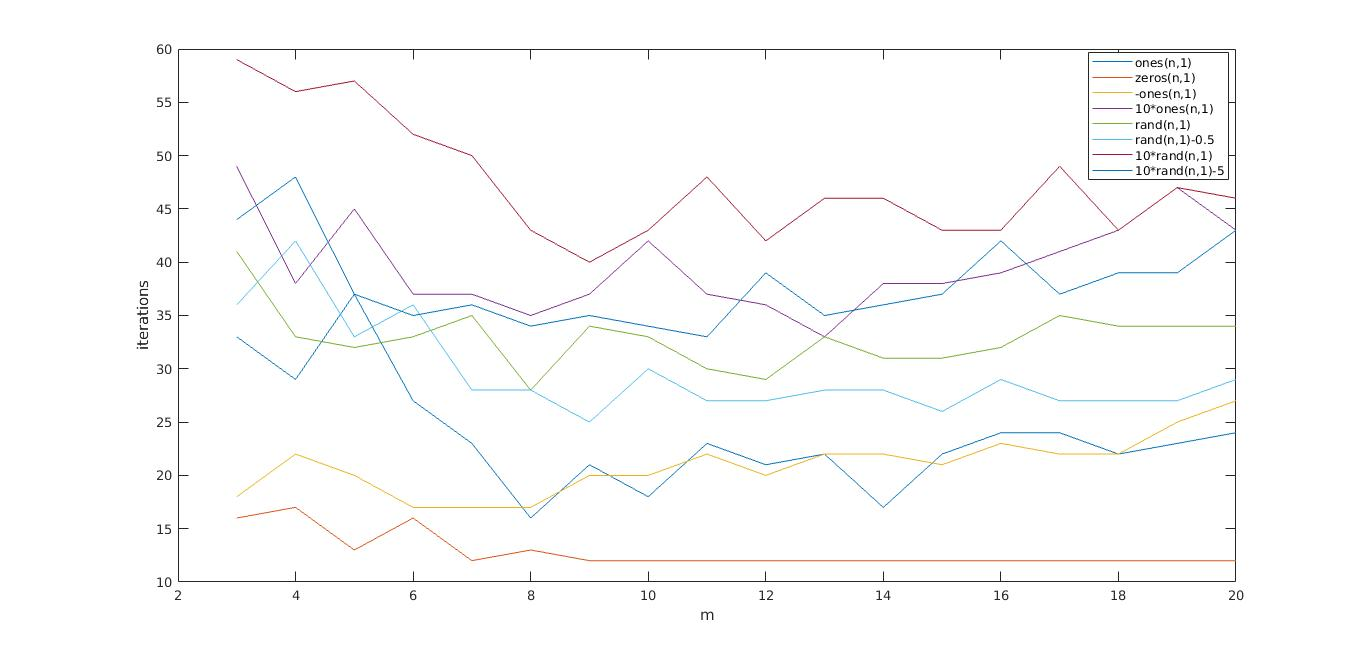
\includegraphics[width=16cm]{matlab/prob6.jpg}
}
\centering
\caption{A plot of iter($m$) with different starting points.}
\end{figure}
Here we comment on the change of the number of iterations, with LBFGS, as a function of $m$ with different starting points. We can see from Figure 1 that $\begin{bmatrix}0 & 0 &\cdots&0 \end{bmatrix}^T $ leads to the smallest number of iterations, and the number of iterations needed oscillates a bit when $m<8$, and it flattens out when we have larger $m$s. For other starting points, it seems that the farther the starting point from the origin is, the more iterations will be needed. We also see an improvement as we increase $m$ in the region of small $m$s, and then we see an oscillating behavior. Generally, regardless of the starting point, $m=8-10$ will get us satisfactory performance.

\subsection{}
After making minor adjustments so that the nonlinear CG methods and BFGS are using the same set of parameters, EBLS script, and starting point (\texttt{ones(100,1)} and \texttt{rand(100,1)}), the following is a table of the results:
\begin{table}[h]
	\centering
	\caption{Iterations needed in nonlinear CG and BFGS algorithms to achieve $\norm{\nabla f(x)}_2\leq 10^{-6}(1+\abs{f(x)})$}
	\begin{tabular}{|c c c|} 
	\hline 
	Algorithm & Iter(\texttt{ones}) & Iter(\texttt{rand}) \\
	\hline \hline
	CG-FR & 189 & 343\\
	\hline
	CG-PRplus & 317 & 472\\
	\hline
	BFGS & 37 & 173 \\
	\hline
	\end{tabular}
\end{table}
So we see that, with uniform input, BFGS performs much better than the nonlinear CG algorithms; with random input, BFGS still performs better, but to a lesser extent.
\end{document}
